\chapter{Simulation Study} \label{chap:simulation}

\section{Simulation}

\subsection{Conditions}

In order to examine the effectiveness of bayesian GLLAMM model, defined in previous chapters, a $3 \times 2 \times 2$ simulation design was performed. The design involved the following conditions:
%
\begin{itemize}
	%
	\item \textbf{Sample size.} the author used three sample sizes: $500$, $250$, and $100$. The data was generated following the algorithm in section \ref{sub_sect:algorithm}. The parameters remained unchanged throughout the simulations.
	%
	\item \textbf{Models.} as defined in figures \ref{fig:FOLV_model} and \ref{fig:SOLV_model}.
	%
	\item \textbf{Parametrization.} it considered the centered (CP) and non-centered parametrization (NCP). 
	%
\end{itemize}

ten ($10$) data sets were generated for each study condition. Each data set resembled responses to $25$ items scored on binary scale, conforming to a second-order latent variable model (SOLV) as defined by figure \ref{fig:SOLV_model}. The model was motivated by the hypothesized structure for the real educational data set corresponding to teacher assessments (see chapter \ref{chap:application}). The latent structure remained unchanged
%
\begin{figure}[h]
	\centering
	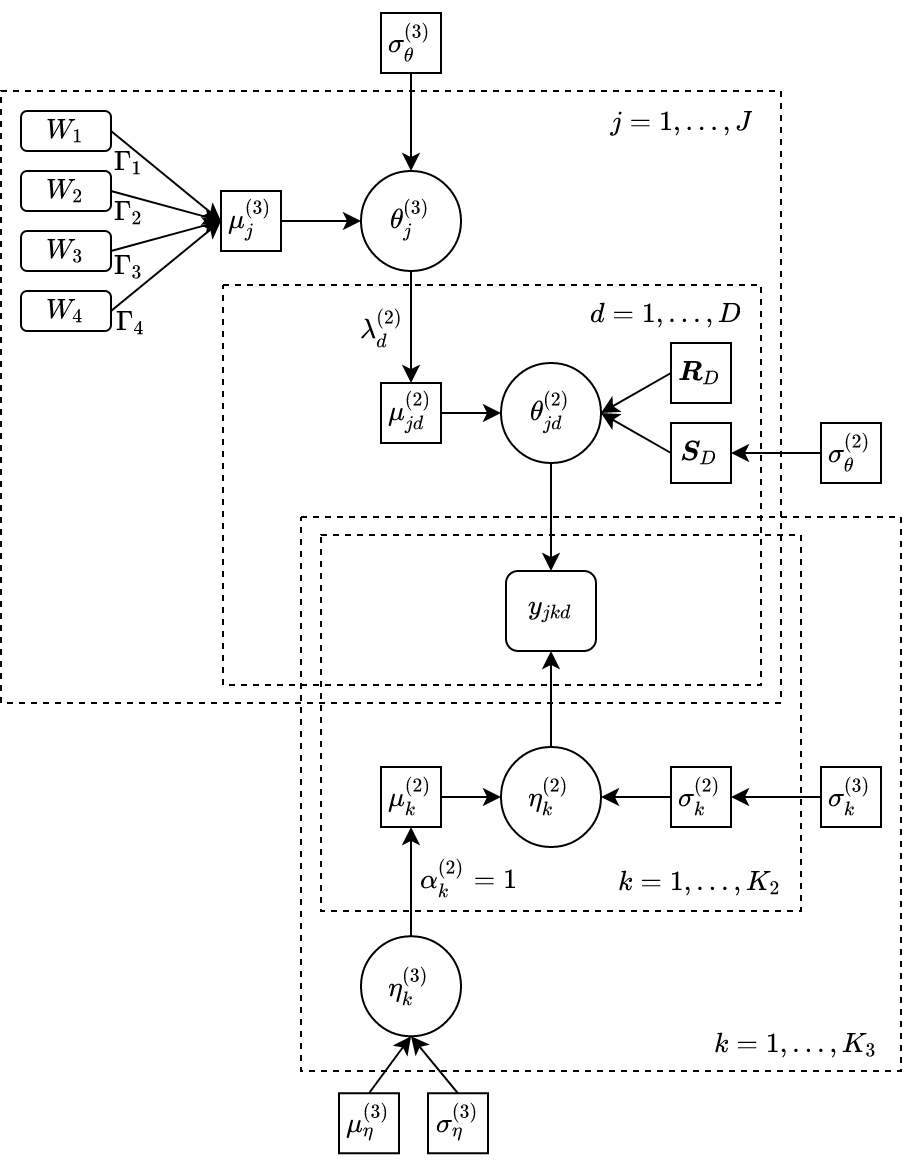
\includegraphics[width=0.7\linewidth]{4_SOLV_dag}
	%
	\caption[Directed Acyclic Graph (DAG). Second Order Latent Variables model (SOLV).]%
	{Directed Acyclig Graph (DAG). Second Order Latent Variables model (SOLV). Circles represent latent variables. Squares represent parameters for priors. Large Squares represent nesting in specific units.}
	\label{fig:SOLV_model}
\end{figure}


%%%%%%%%%%%%%%%%%%%%%%%%%%%%%%%%%%%%%%%%%%%%%%%%%%%%%%%%%%%%%%%%%%%%%%%

\subsection{Algorithm} \label{sub_sect:algorithm}

the data was simulated from the latent structure as defined by figure \ref{fig:SOLV_model} following the next steps:

\begin{enumerate}	
	%
	\item \textbf{Covariates:} four pseudo-covariates were simulated motivated for the real data set. We report also their regression parameters:
	%
	\begin{enumerate}
		%
		\item \textit{gender}, binary variable. $\beta_{G}=[\beta_{G(1)}, \beta_{G(2)}] = [0, 1]$
		%
		\item \textit{age}, integer variable with range $[30, 65]$, $\beta_{Ac} = -0.01$
		%
		\item \textit{education}, categorical variable with three categories. $\beta_{E}=[\beta_{E(1)}, \beta_{E(2)}, \beta_{E(3)}] = [-0.5, 0.5, 0]$
		%
		\item \textit{experience}, categorical variable with four categories. $\beta_{X}=[\beta_{X(1)}, \beta_{X(2)}, \beta_{X(3)}] = [-0.5, 0, 0.35, 0.5]$
		%
	\end{enumerate}
	%
	\item \textbf{Dimensions:} 
	%
	\begin{enumerate}
		%
		\item \textit{one SOLV} was generated by a normal distribution with a mean defined by a linear combination of the simulated covariates and its corresponding regression parameters. Additionally it assumed a standard deviation $\sigma^{(3)}_{\theta}=0.5$.
		%
		\item \textit{three FOLV} are generated by a multivariate normal distribution with a mean vector defined by multiplying the loadings $[0.95, 0.95, 0.95]$ times the simulated SOLV $\theta_{j}$. It was assumed the three FOLV were independent between each other after consider the influence the higer-level latent variable, therefore the covariance matrix was defined as a diagonal matrix with diagonal $\sigma^{(2)}_{\theta}=0.5$.
		%
	\end{enumerate}
	%
	\item \textbf{Items:} 
	%
	\begin{enumerate}
		%
		\item \textit{texts} the mean difficulty for $5$ texts was defined in the following way: $\eta^{3}_{k} = [-1.50, -0.75, 0, 0.75, 1.50]$. While the deviation form the mean difficulty was assumed $\sigma^{(3)}_{\eta}=0.5$
		%
		\item \textit{25 items} were generated from independent normal distribution with mean equal to the mean difficulty and deviation equal to the deviation corresponding to their respective texts. We made the items pointed out to one of the three latent dimension by random sample.
		%
	\end{enumerate}
	%
	\item \textbf{Probabilities:} the probability $\pi_{jkd}$ was calculated through the logit inverse-link function as defined in equation (\ref{eq:systematic}) and (\ref{eq:response_dich1}).
	
	\item \textbf{Outcome:} the outcome is simulated from a Bernoulli distribution as in equation (\ref{eq:distributional}), with probability calculated in the previous step.
\end{enumerate}

\noindent The code associated with the full simulation process can be found in Appendix \ref{appC2_1:sim}. \\



%%%%%%%%%%%%%%%%%%%%%%%%%%%%%%%%%%%%%%%%%%%%%%%%%%%%%%%%%%%%%%%%%%%%%%%
%%%%%%%%%%%%%%%%%%%%%%%%%%%%%%%%%%%%%%%%%%%%%%%%%%%%%%%%%%%%%%%%%%%%%%%

\section{Evaluation criteria}

La precisión de los estimados fue evaluada usando la Raíz del Error Cuadrático Medio (RMSE) y el Error Absoluto Medio (MAE) para cada réplica (acorde con los diseños establecidos en \ref{sec:cond_simulacion}). \\

El RMSE es definido como la raíz cuadrada del promedio de las diferencias entre los valores reales y los estimados al cuadrado, de la siguiente manera:
\begin{align}
	%
	RMSE \left( \eta^{(m)}_{kd} \right) &=\sqrt{\frac{1}{R} \sum_{r=1}^{R} (\hat{\eta}^{(m)}_{kd} - \eta^{(m)}_{kd} )^2} \\
	%
	RMSE \left( \theta^{(l)}_{jd} \right) &=\sqrt{\frac{1}{R} \sum_{r=1}^{R} (\hat{\theta}^{(l)}_{jdr}-\theta^{(l)}_{jd})^2}
	%
\end{align}

Tal y como se observa en las fórmulas, los criterios serán aplicados a los parámetros de ítem e individuos. Sin embargo, dado que en el NRM, el impacto de cada categoría depende ampliamente de los valores y comportamiento de las otras, en determinados casos se podría observar diferencias entre el parámetro real y estimado que no necesariamente corresponderían con un error en la estimación de la elección de la categoría por parte del individuo \citep{Wollack2002}. Así, para corregir este inconveniente se comparará no solo los estimados de los parámetros de los ítems e individuos, sino también las probabilidades condicionales asociadas a la elección de cada alternativa específica \cite{Yen_1987, Wollack_2002}. De este modo, dado que las probabilidades $P_{jk}(\theta_{i})$ difieren entre sí, no solo por los parámetros de los ítems ($a_{jk}$ y $c_{jk}$) sino también en función de las habilidades ($\theta_i$), para el análisis de las diferencias entre las probabilidades estimadas y las reales, se planteó utilizar los dos criterios (RMSE y MAE) con algunos ajustes:

\begin{align}
	%
	RMSE \left( \pi_{jkd} \right) &=\sqrt{ \frac{1}{n} \sum_{i=1}^{n} \left[ \frac{1}{R} \sum_{r=1}^{R} (\hat{\pi}_{jkdr} - \pi_{jkd})^2 \right]} \\
	%
\end{align}

\noindent donde $\hat{\pi}_{jkdr}$ es el estimado de las probabilidades condicionales en la réplica $r = 1, \dots, R$.\\

\noindent Como se observa en las formulas $(4.7)$ y $(4.8)$, las diferencias entre probabilidades se agregan y promedian a nivel de replicas y posteriormente a nivel de individuos en cada una de las réplicas ($R=20$). De esta manera, se tienen una medida global de ajuste a los datos. \\


additionally we are going to use predictive accuracy, sensitivity and the other
binary case. Based on a confussion matrix 


%%%%%%%%%%%%%%%%%%%%%%%%%%%%%%%%%%%%%%%%%%%%%%%%%%%%%%%%%%%%%%%%%%%%%%%
%%%%%%%%%%%%%%%%%%%%%%%%%%%%%%%%%%%%%%%%%%%%%%%%%%%%%%%%%%%%%%%%%%%%%%%

\section{Results}

following the CFA model construction we are going to evaluate two models that can be considered equivalent 
%
\begin{figure}[h]
	\centering
	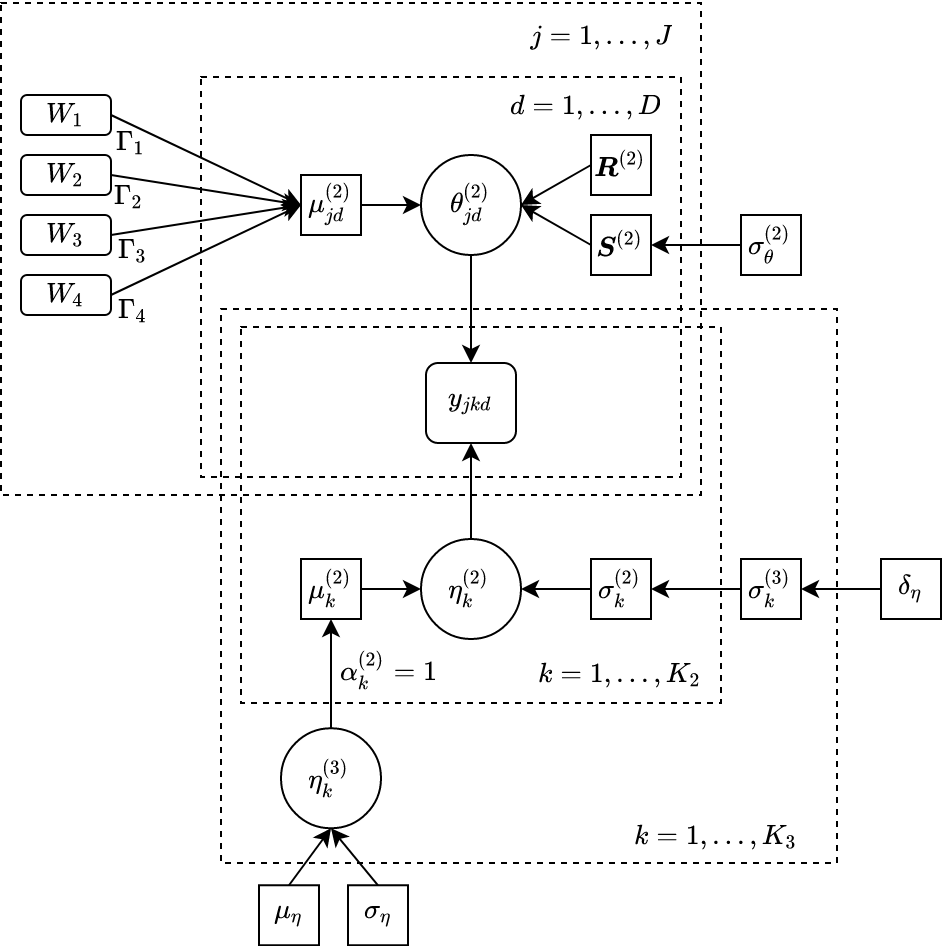
\includegraphics[width=0.7\linewidth]{4_FOLV_dag}
	%
	\caption[Directed Acyclig Graph (DAG). First Order Latent Variables model (FOLV).]%
	{Directed Acyclig Graph (DAG). First Order Latent Variables model (FOLV). Circles represent latent variables. Squares represent parameters for priors. Large Squares represent nesting in specific units.}
	\label{fig:FOLV_model}
\end{figure}


\subsection{FOLV CP}

\subsection{FOLV NCP}

\subsection{SOLV CP}

\subsection{SOLV NCP}

